\documentclass[11pt,a4paper]{article}
\usepackage[margin=23mm]{geometry}
\usepackage{booktabs,graphicx,amsmath,hyperref}
\hypersetup{colorlinks=true,urlcolor=blue}
\graphicspath{{../../docs/results/velocity-class-control/}}
\setlength{\parindent}{0pt}\setlength{\parskip}{5pt}
\newcommand{\record}[2]{\href{https://github.com/LiuJingting0201/cnr-road-gaf-diffusion/blob/main/docs/results/#1}{#2}}
\begin{document}
{\small MASTER'S THESIS PROGRESS REPORT \hfill 17 November 2026}

{\LARGE\bfseries How does speed enter trajectory diffusion?\par}
Jingting Liu

\textbf{Finding.} A bus and a bicycle can finish a journey at the same average speed while spending very different amounts of time moving slowly. On five-class SUMO data, a DiffTraj model that generated velocity vectors recovered much more of this difference than one that generated coordinates. Its trajectories also missed the requested destination cell more often. This report follows the experiments that established both results.

\section*{1. Adding speed to coordinate diffusion}
The starting point was \href{https://proceedings.neurips.cc/paper_files/paper/2023/hash/cd9b4a28fb9eebe0430c3312a4898a41-Abstract.html}{DiffTraj (Zhu et al., NeurIPS 2023)}. Given trip attributes, its denoiser learns to remove Gaussian noise from a sequence of 200 positions. The request already gives the trip-average speed. Our question was whether information about speed \emph{within} the trip would improve the motion reconstructed from successive generated positions.

An exploratory Beijing GeoLife experiment provided an initial motivation. In 108 matched bus--bicycle pairs, the observed low-speed time shares differed by 16.3 percentage points. Adding training penalties for low-speed share and entry rate to a class-conditioned coordinate model produced a label-switch difference below 0.01 points in both seeds. We used a larger, balanced SUMO corpus for the controlled comparisons below. \record{beijing-rhythm/REPORT.md}{Beijing results}

\textbf{During training.} We compared two coordinate models with the same vehicle labels. One also penalized differences between predicted and observed segment speeds on the training trip. The extra term improved bicycle and motorcycle speed distributions at both seeds, while bus and taxi deteriorated. Across the five equally weighted classes, the average speed error increased.

\textbf{During sampling.} We then froze the coordinate model. For each request we retrieved 32 same-class training trips with similar duration and mean speed. Five quantiles of their speeds guided the denoising steps. This improved speed W1 for every class at both seeds, with little change in the spatial metrics.

\begin{center}\small
\begin{tabular}{lrr}\toprule
Five-class mean speed W1 (m/s), lower is better & Seed 42 & Seed 43\\\midrule
Coordinate diffusion, standard sampler & .917 & .883\\
With segment-speed training loss & .958 & .890\\
With speed-quantile sampling guidance & .871 & .836\\\bottomrule
\end{tabular}\end{center}
W1 is the first Wasserstein distance between generated and observed speed distributions. Quantiles describe how often different speeds occur. They do not encode their order. In a bus diagnostic, shuffling the observed speeds within each trip preserved the speed distribution exactly while reducing the median low-speed spell from 29.0 to 13.1 seconds. That motivated testing the entire velocity sequence as the diffusion target. \record{general-speed-class/REPORT.md}{Five-class comparisons} $\cdot$ \record{terminal-bus/REPORT.md}{Bus diagnostic}

\newpage
\section*{2. Generating velocities and integrating a trip}
We simulated complete journeys on the MoST network in SUMO. Buses followed predefined routes with stops. Bicycles, motorcycles, passenger cars and taxis drew origins and destinations from roads permitted for their class. We retained completed trips with at least 120 consecutive one-second positions and interpolated each journey to 200 positions over its own duration $T$. The five classes supplied 40,000 training trips each. Validation used different simulation episodes.

For positions $p_0,\ldots,p_{199}$ in metres, we computed the two-dimensional velocity $v_i=(p_i-p_{i-1})/\Delta t$, where $\Delta t=T/199$. The velocity model generated a starting offset within the origin-cell coordinate system and 199 velocity vectors. From the sampled start $\hat p_0$ we recovered the positions by summation,
\[
\hat p_j=\hat p_0+\Delta t\sum_{i=1}^{j}\hat v_i .
\]
The two components retain direction, so the model can turn. An error in the sum of those components displaces the endpoint even when the individual speed magnitudes look plausible.

\textbf{Single-class check.} On 1,000 taxi validation requests, switching from coordinates to velocities reduced speed W1 from 1.183/1.173 to 0.160/0.203 m/s (seeds 42/43). Destination-cell hits dropped from 72.6/73.1\% to 31.1/32.6\%. This established a motion--location trade-off before introducing vehicle labels. \record{velocity-diffusion-pilot/REPORT.md}{Taxi comparison}

\textbf{Five-class test.} We trained both representations from scratch with the same labelled 200,000 trips, U-Net, noise-prediction loss and trainable class embedding. Both received departure time, distance, duration, point count, mean displacement, mean speed and origin/destination cells. Each fit used 10 epochs, batch 205, 9,760 AdamW updates, norm-1 gradient clipping and cosine learning-rate decay from $2\,10^{-4}$ to $2\,10^{-5}$. Each representation used seeds 42 and 43. We sampled final checkpoints with 100 DDIM steps. This comparison has its own coordinate control because the earlier supervision experiment used a different training schedule.

\begin{center}\small
\begin{tabular}{lrr}\toprule
Five-class validation mean & Coordinates (42 / 43) & Velocities (42 / 43)\\\midrule
Speed W1 (m/s) $\downarrow$ & 1.213 / 1.080 & .212 / .179\\
Acceleration W1 (m/s$^2$) $\downarrow$ & .181 / .190 & .027 / .032\\
Point density JS $\downarrow$ & .0077 / .0078 & .0371 / .0408\\
Origin--destination JS $\downarrow$ & .2357 / .2448 & .3398 / .3470\\
Trip length JS $\downarrow$ & .0310 / .0253 & .0213 / .0112\\
Hotspot F1 $\uparrow$ & .950 / .930 & .800 / .820\\
Destination cell hit $\uparrow$ & 71.7 / 70.5\% & 38.2 / 37.7\%\\\bottomrule
\end{tabular}\end{center}
The table uses 600 fixed validation requests per class. Speed and tangential acceleration are computed from the reconstructed positions on the same physical-time grid as the observed comparison. Jensen--Shannon divergence (JS) compares occupancy, OD-pair or length histograms. Hotspot F1 measures overlap among the 20 busiest grid cells. The destination hit checks each trip against its requested cell. \record{velocity-class-control/STATS.md}{Per-class scores and evaluation details}

\newpage
\section*{3. Does changing the label change the way a vehicle moves?}
We kept each request, including its mean speed, and the initial diffusion noise fixed, and changed only the vehicle label. To determine whether the generated change pointed in a realistic direction, we compared it with observed SUMO trips matched on similar requests. For buses and bicycles, 53 observed pairs had requested mean speeds within 0.50 m/s of one another. The mean signed gap was only $-0.074$ m/s. The observed contrast includes route and service differences on this network.

\begin{center}\small
\begin{tabular}{lrrr}\toprule
Bus minus bicycle & SUMO & Coordinates (42 / 43) & Velocities (42 / 43)\\\midrule
Time below 1 m/s (percentage points) & +39.6 & +2.54 / +2.90 & +26.1 / +25.1\\
Low-speed entries per 10 min & +7.87 & +0.54 / +0.74 & +5.40 / +5.13\\
90th-percentile speed (m/s) & +7.38 & +1.00 / +0.89 & +5.35 / +5.14\\
Mean absolute acceleration (m/s$^2$) & +.363 & +.074 / +.050 & +.268 / +.254\\\bottomrule
\end{tabular}\end{center}
The velocity model recovered about two thirds of the observed low-speed time and entry differences. A low-speed entry requires at least two consecutive intervals below 1 m/s after a faster interval. A second contrast concerned acceleration: in 253 matched pairs, passenger cars had lower mean absolute acceleration than motorcycles by 0.093 m/s$^2$. The velocity model recovered reductions of 0.070/0.074 m/s$^2$. Passenger cars and taxis showed little observed separation, and six of the ten class pairs retained at most 12 matches under the strict mean-speed rule. \record{velocity-class-control/BALANCE.md}{All matching counts and uncertainty intervals}

\begin{center}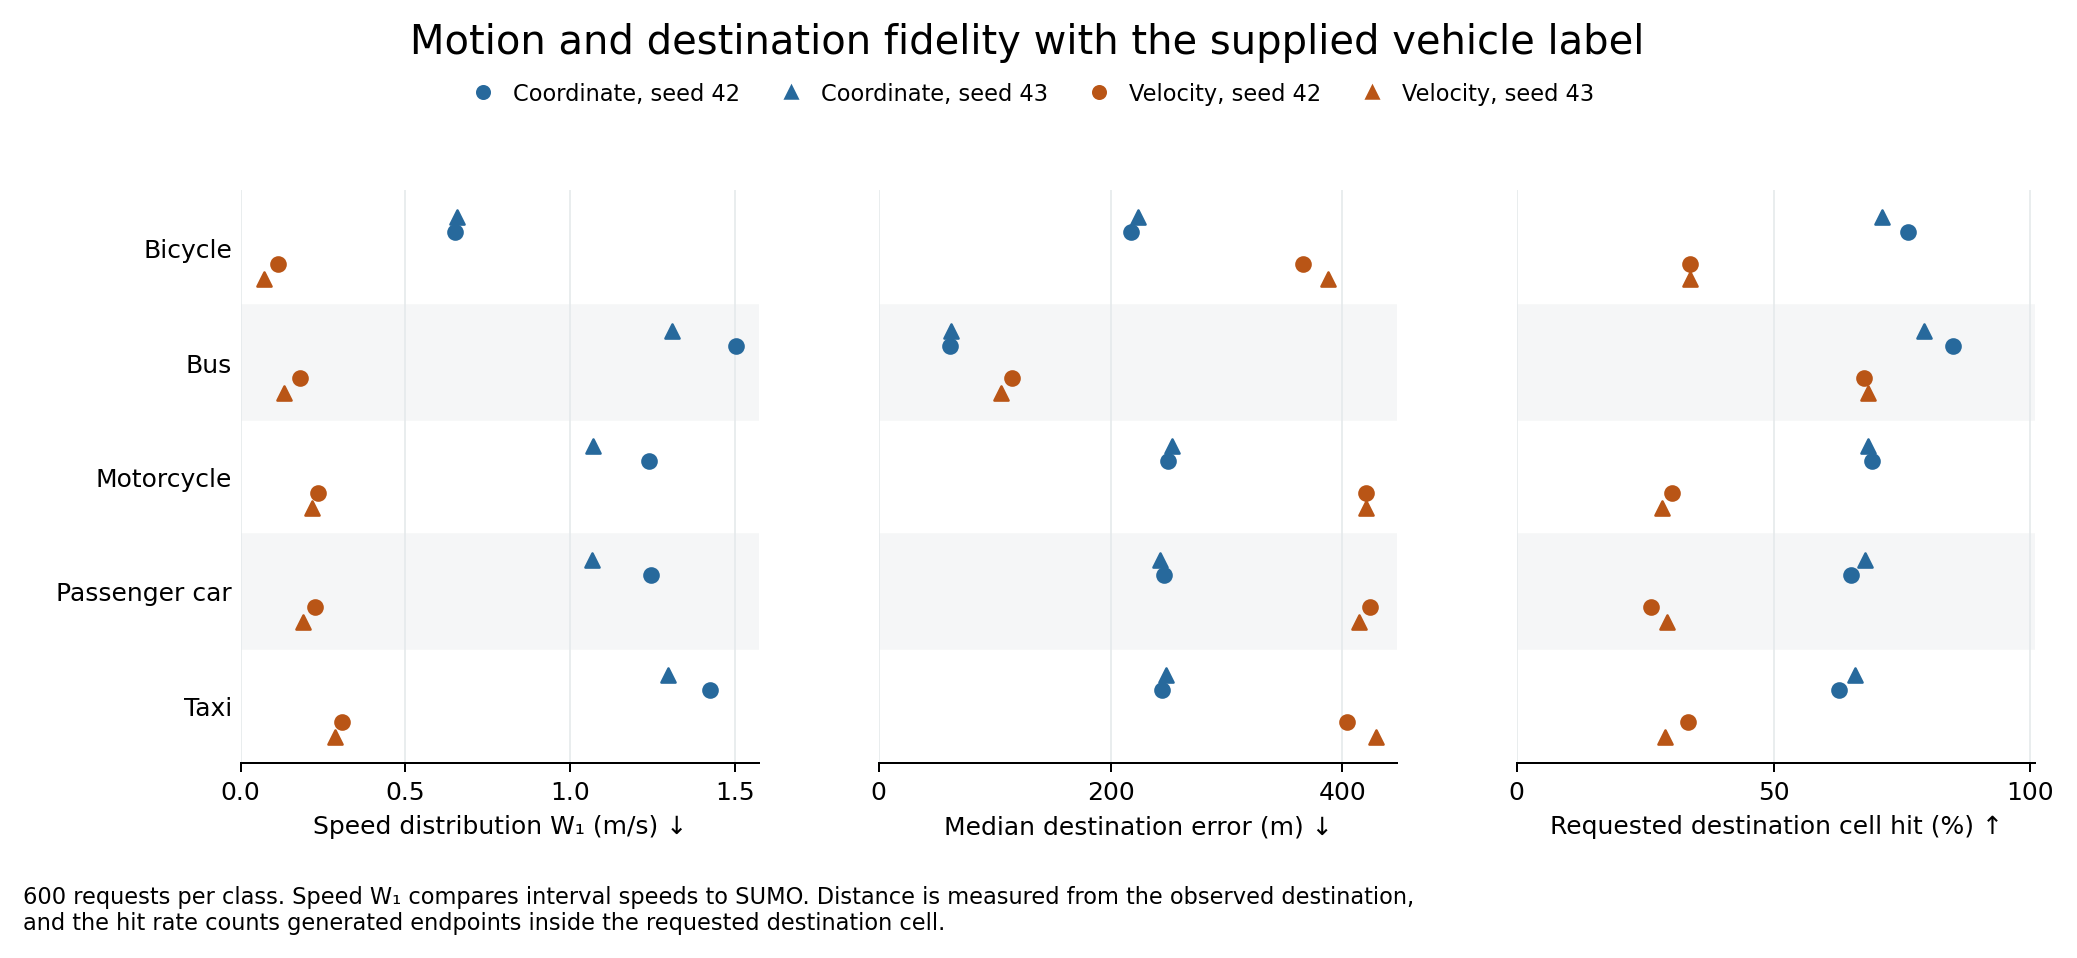
\includegraphics[width=.98\linewidth]{motion-and-endpoints.png}\end{center}
{\small Figure 1. The velocity model reduced speed-distribution error in every vehicle class at both seeds. The centre and right panels show the corresponding increase in median distance to the observed endpoint and the drop in requested-cell hits.}

\textbf{Does supplying the class help at sampling time?} As a check, we inferred a plausible class from similar training requests instead of supplying the recorded label. This already selected the correct class for 1,826 of 3,000 requests. Supplying the recorded class reduced the velocity model's speed W1 by a further 0.024/0.038 m/s. The modest average gain and the larger fixed-request bus--bicycle effect answer different questions: many requests already reveal their likely class, yet deliberately switching class can change how a particular trip unfolds.

\newpage
\section*{4. What one generated trip looks like}
\begin{center}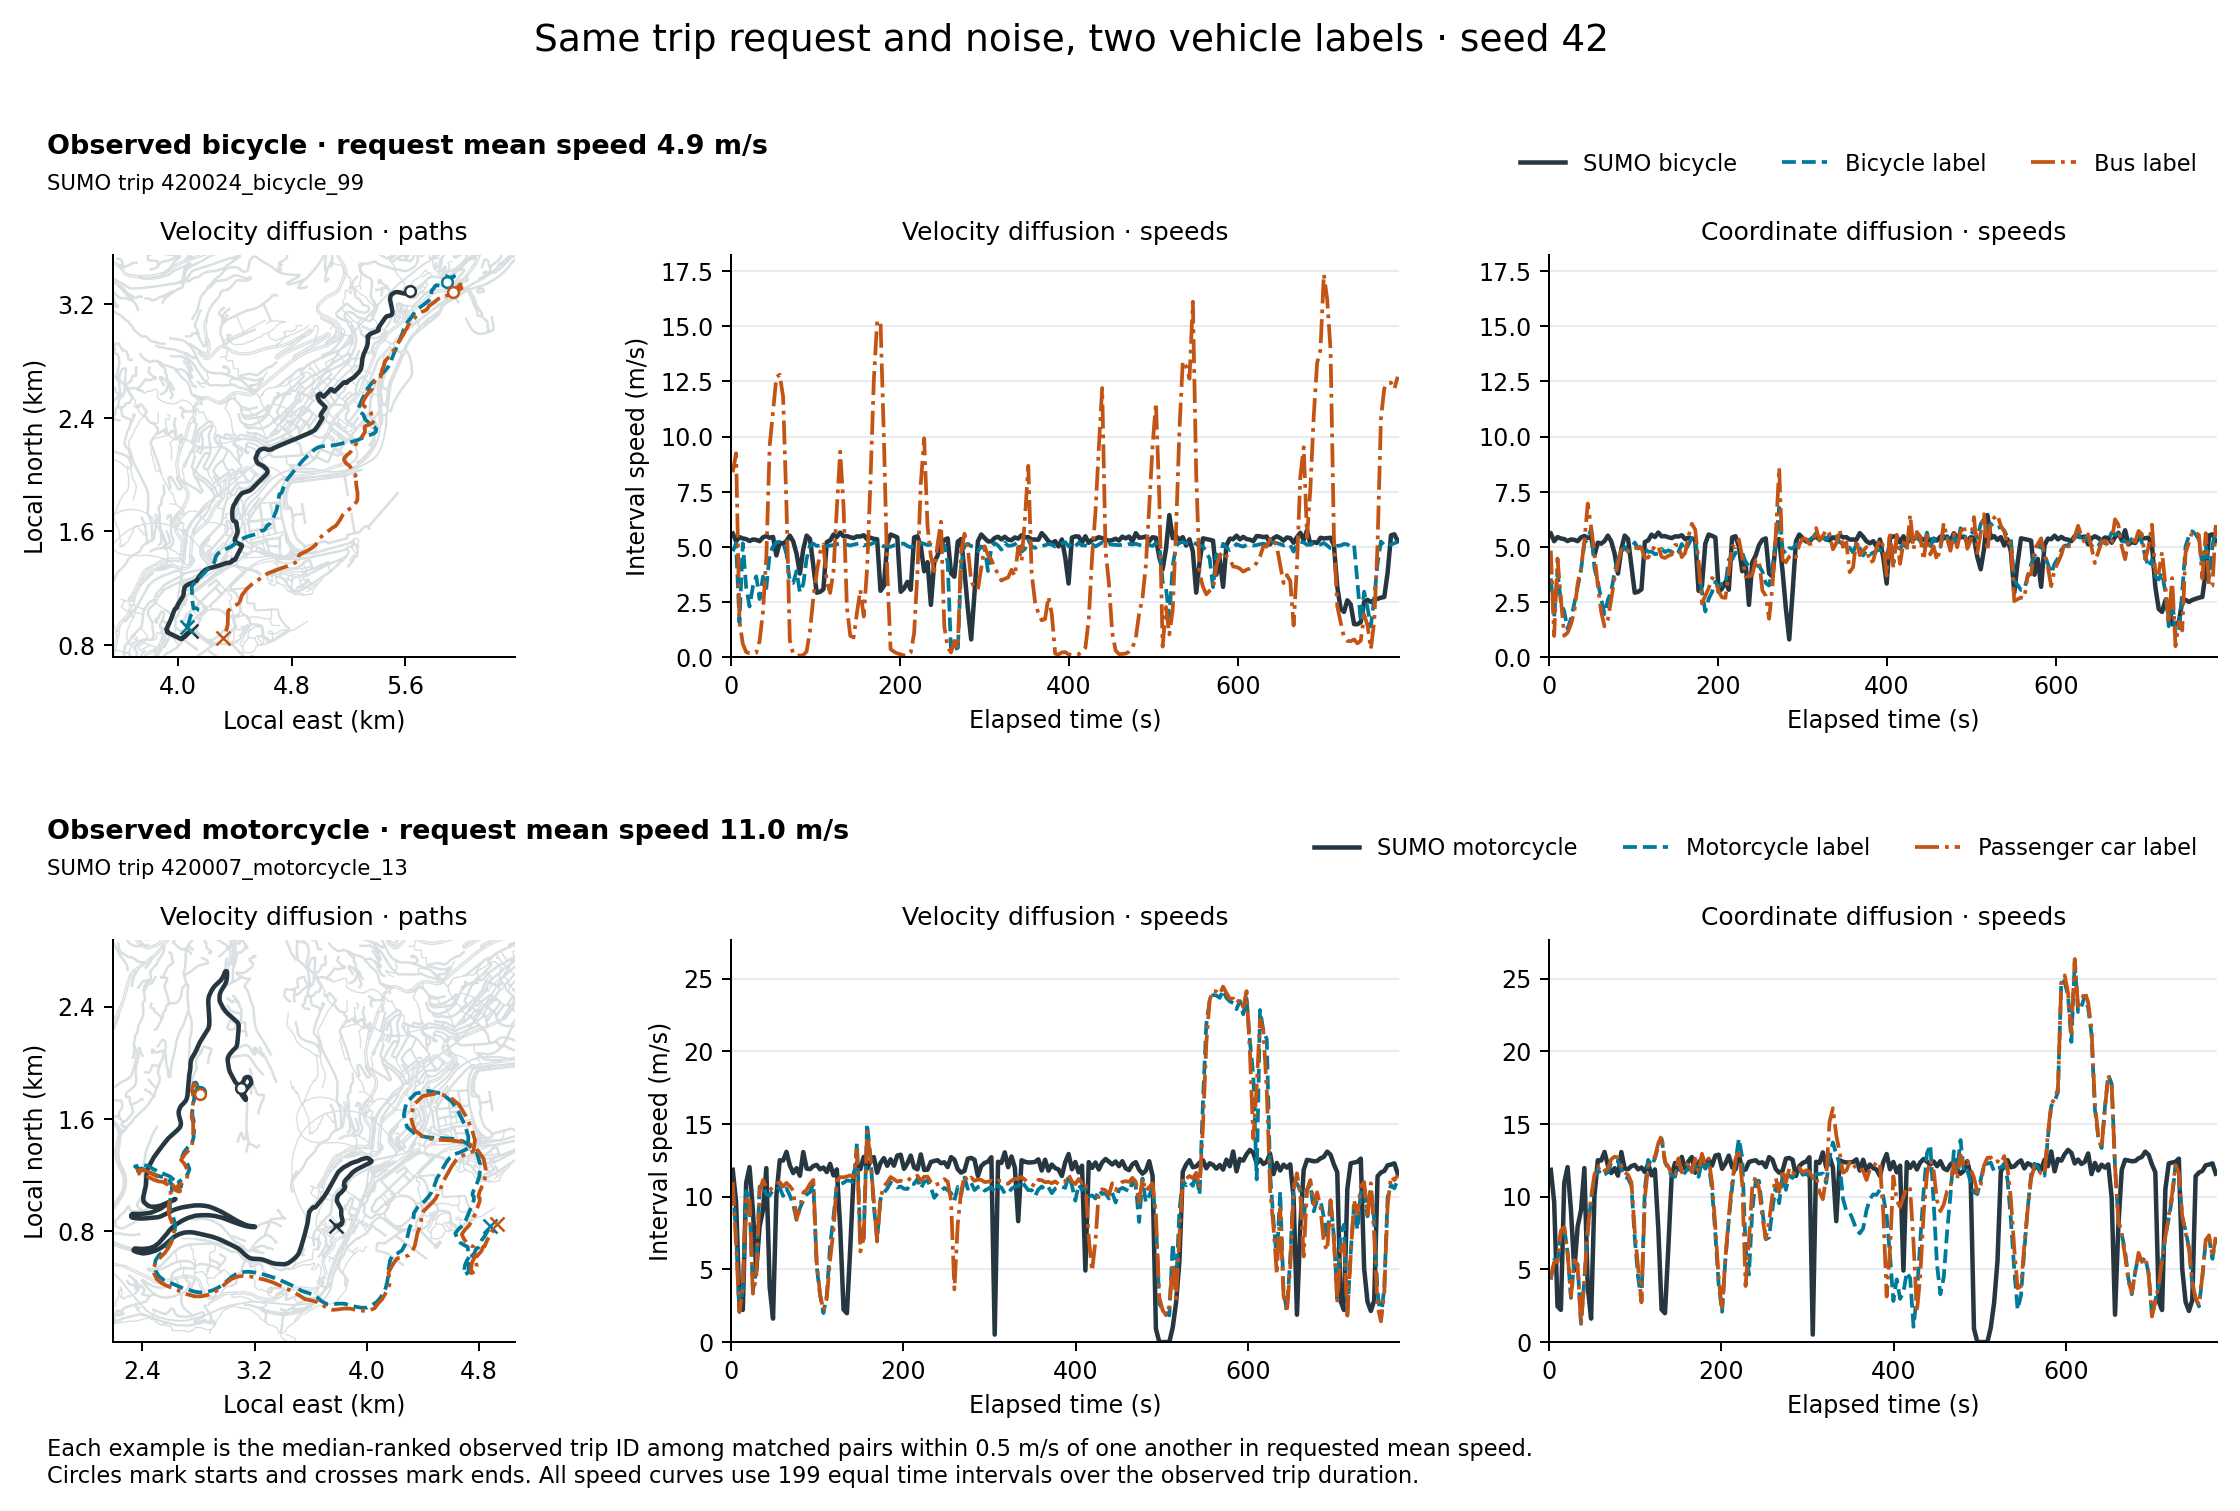
\includegraphics[width=\linewidth]{trips-42.png}\end{center}
{\small Figure 2. Two requests selected by median trip-ID rank among eligible matches. In the first row the requested mean is 4.9 m/s. With the velocity model, changing bicycle to bus produces repeated slow periods and higher moving speeds. The coordinate model produces similar curves for both labels. The maps show that a plausible speed profile can still lead to a misplaced destination. \record{velocity-class-control/trips-43.png}{Same requests at seed 43}.}

\textbf{Conclusion.} In these SUMO validation experiments, sampling guidance modestly improved the speed distribution. Generating velocities directly produced larger motion gains and let vehicle labels control stop--go behaviour at a fixed requested mean speed. The remaining design question is whether the model can retain that control while reaching the requested destination more reliably.
\newpage\section*{Road maps by vehicle: Bicycle}
Each block shows one validation request under the supplied vehicle label (seed 42). Within a block, the six maps share the same road extent and speed scale. A circle marks the start and a cross the end of each plotted path.
\begin{center}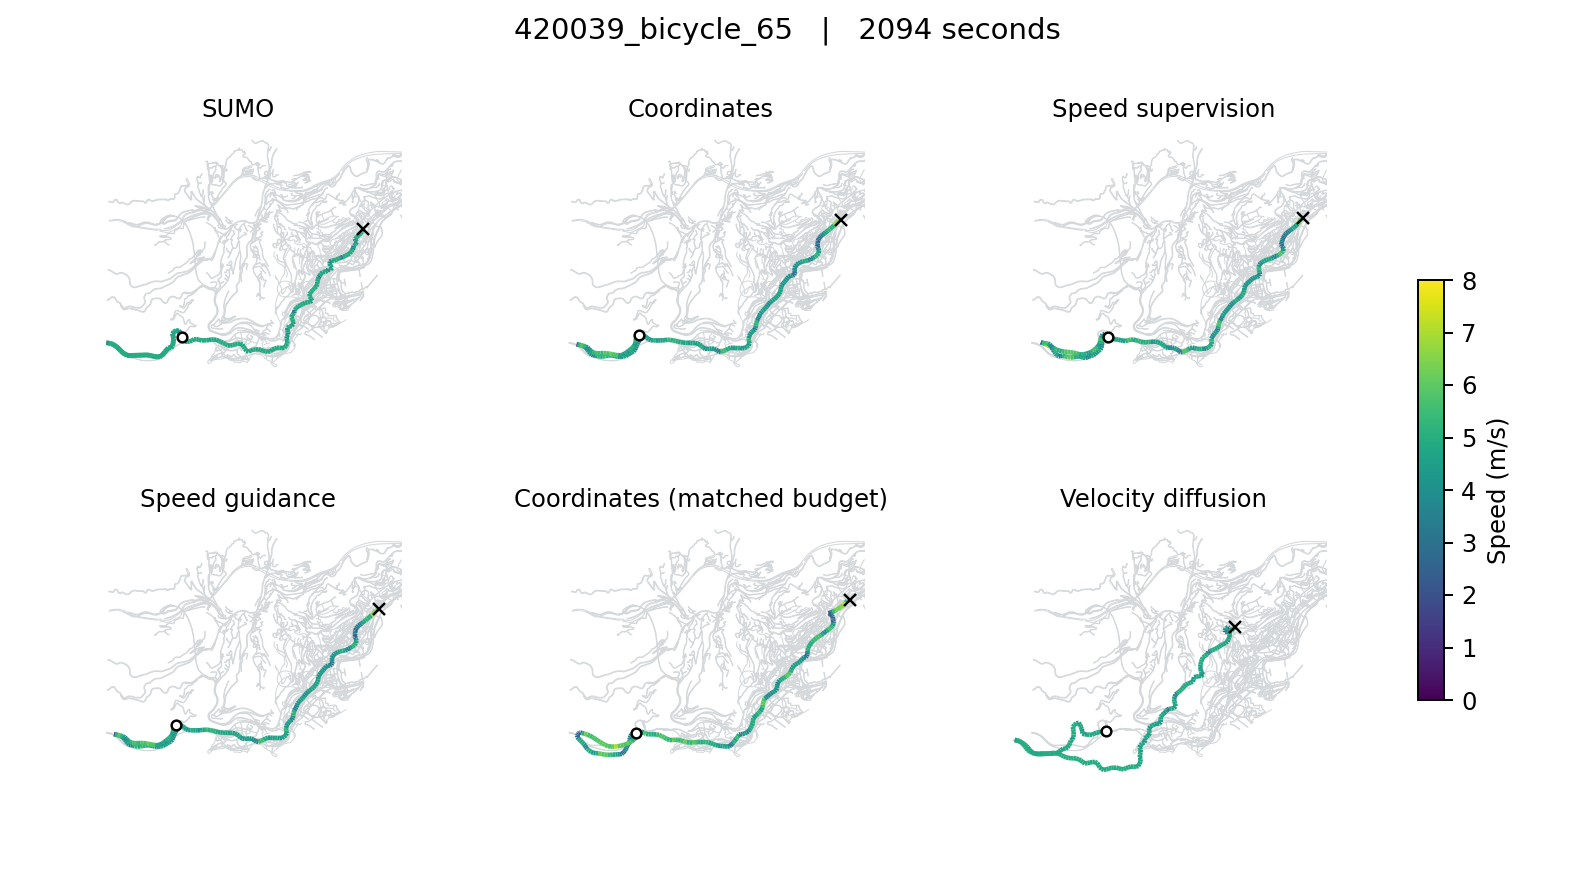
\includegraphics[width=.97\linewidth]{maps/bicycle-1.png}\end{center}
\begin{center}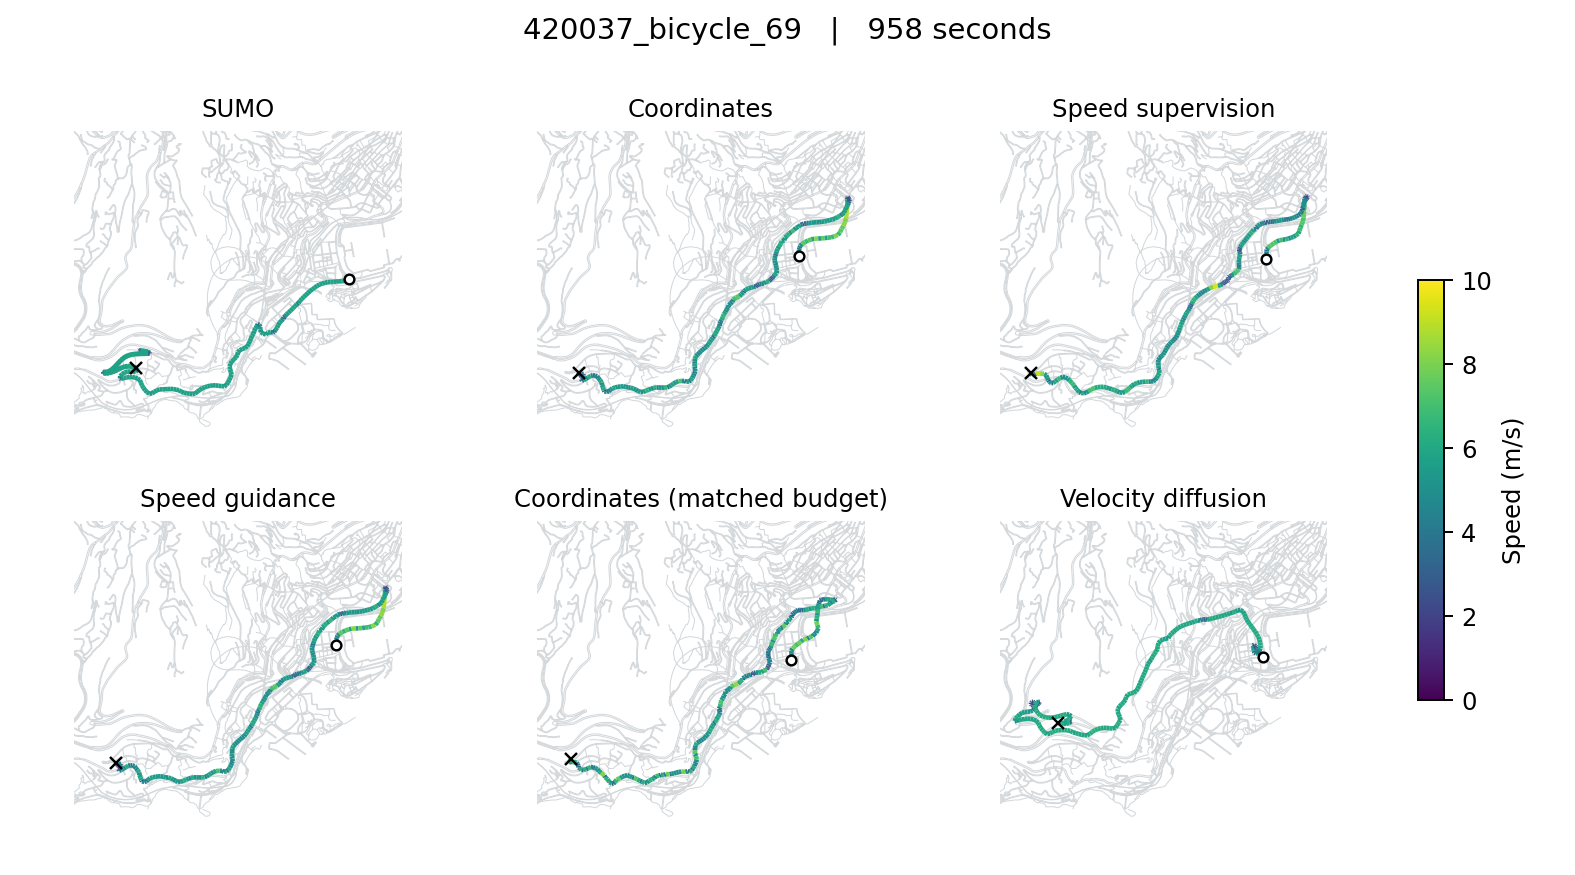
\includegraphics[width=.97\linewidth]{maps/bicycle-2.png}\end{center}
{\small Top row: SUMO, coordinate baseline, speed supervision. Bottom row: speed guidance applied to the top-row baseline, the separately trained coordinate control for velocity diffusion, and velocity diffusion. The first two requests per class in the fixed validation order were selected before viewing the maps.}

\newpage\section*{Road maps by vehicle: Bus}
Each block shows one validation request under the supplied vehicle label (seed 42). Within a block, the six maps share the same road extent and speed scale. A circle marks the start and a cross the end of each plotted path.
\begin{center}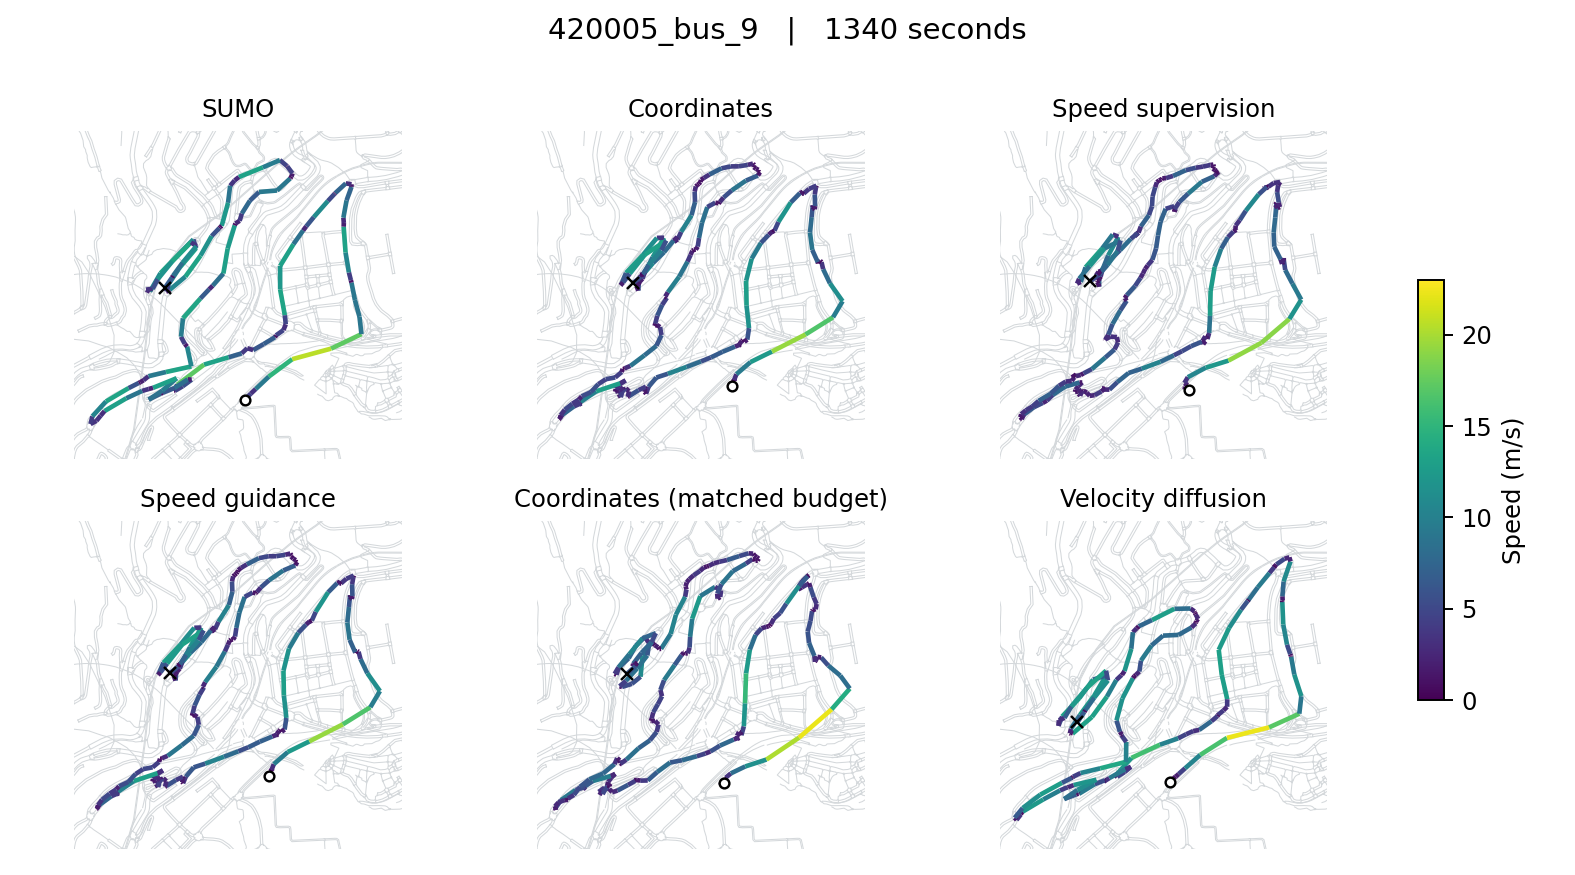
\includegraphics[width=.97\linewidth]{maps/bus-1.png}\end{center}
\begin{center}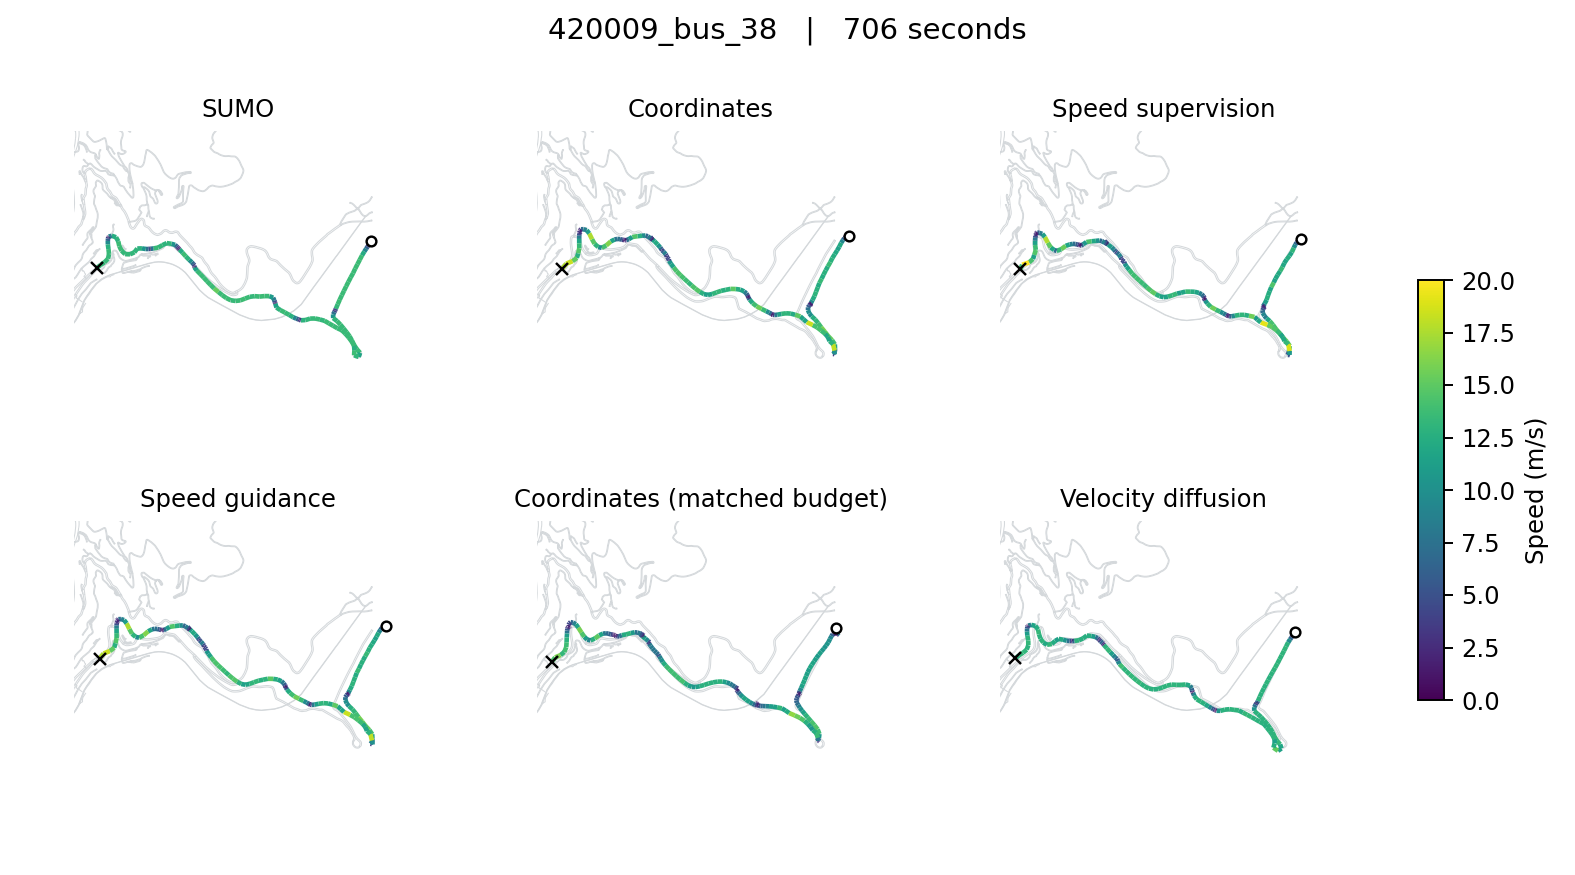
\includegraphics[width=.97\linewidth]{maps/bus-2.png}\end{center}
{\small Top row: SUMO, coordinate baseline, speed supervision. Bottom row: speed guidance applied to the top-row baseline, the separately trained coordinate control for velocity diffusion, and velocity diffusion. The first two requests per class in the fixed validation order were selected before viewing the maps.}

\newpage\section*{Road maps by vehicle: Motorcycle}
Each block shows one validation request under the supplied vehicle label (seed 42). Within a block, the six maps share the same road extent and speed scale. A circle marks the start and a cross the end of each plotted path.
\begin{center}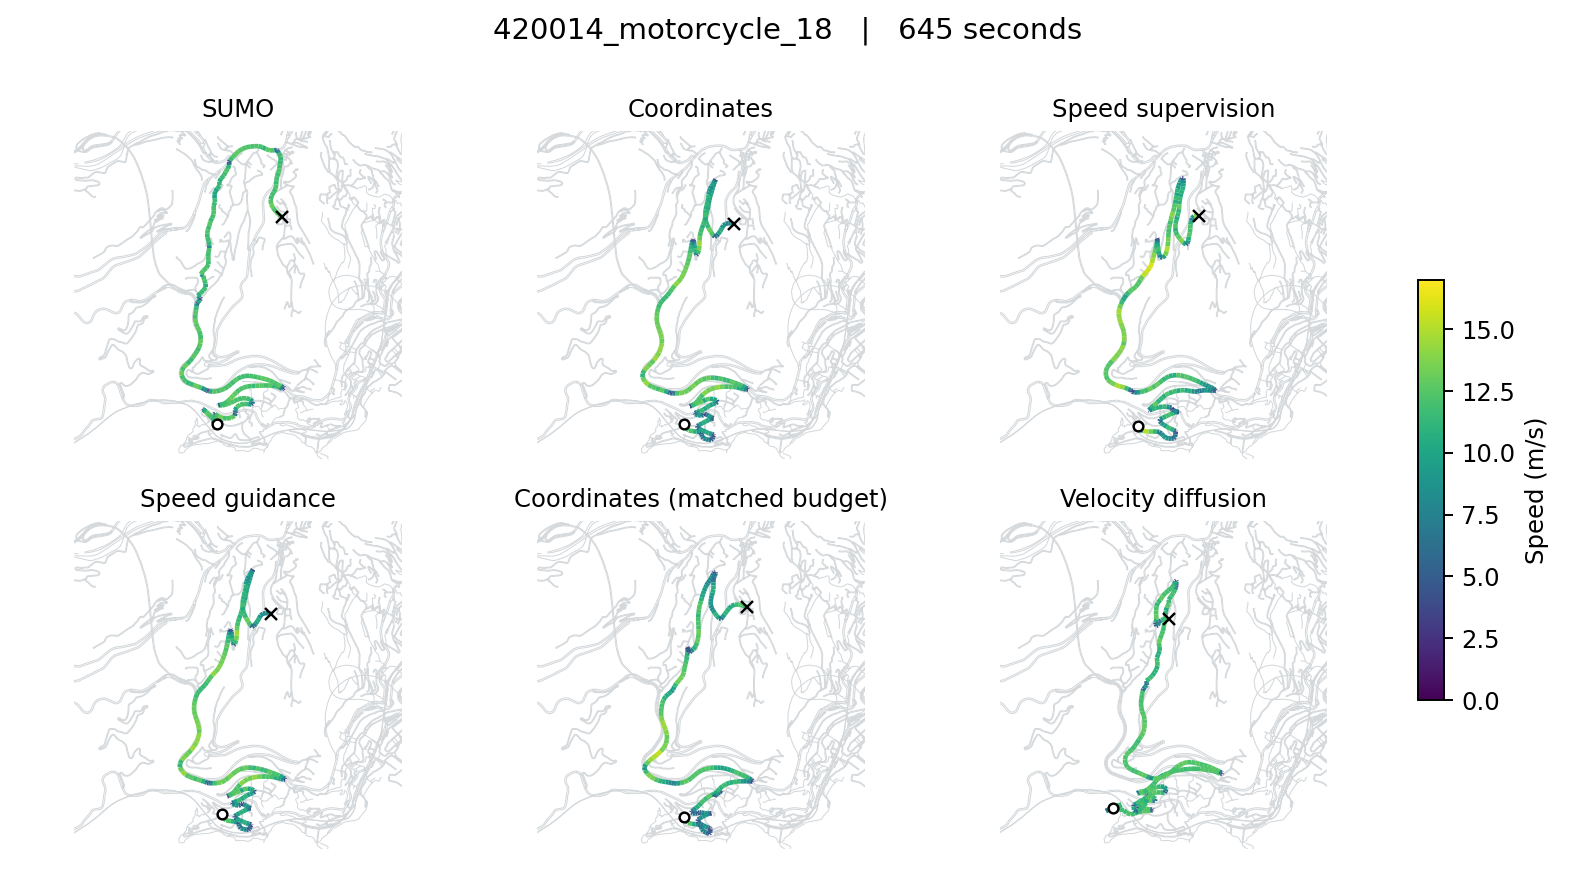
\includegraphics[width=.97\linewidth]{maps/motorcycle-1.png}\end{center}
\begin{center}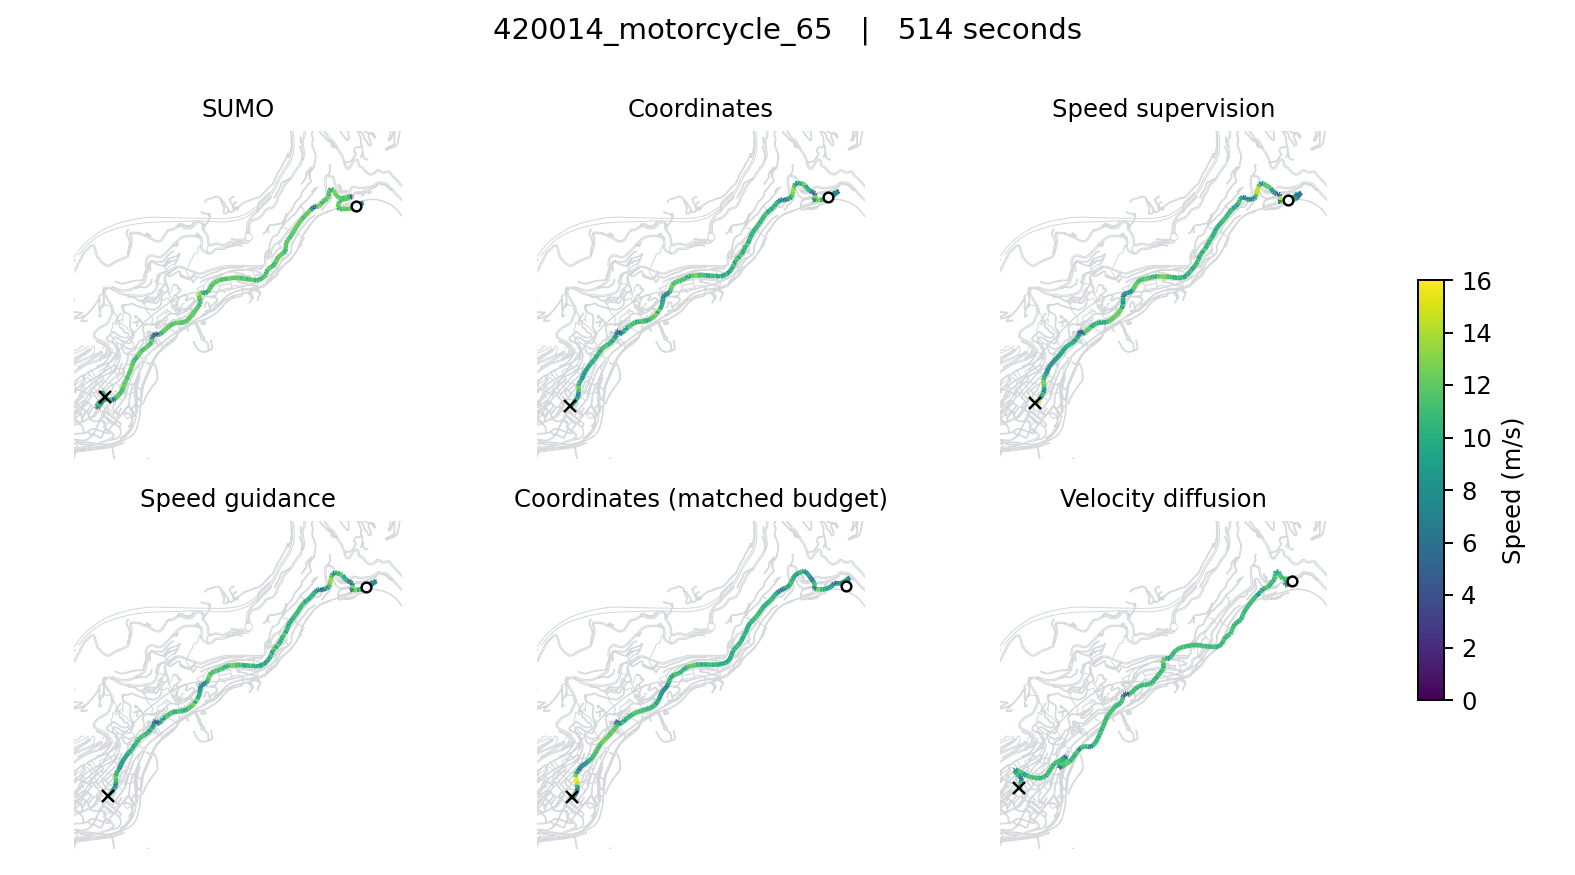
\includegraphics[width=.97\linewidth]{maps/motorcycle-2.png}\end{center}
{\small Top row: SUMO, coordinate baseline, speed supervision. Bottom row: speed guidance applied to the top-row baseline, the separately trained coordinate control for velocity diffusion, and velocity diffusion. The first two requests per class in the fixed validation order were selected before viewing the maps.}

\newpage\section*{Road maps by vehicle: Passenger car}
Each block shows one validation request under the supplied vehicle label (seed 42). Within a block, the six maps share the same road extent and speed scale. A circle marks the start and a cross the end of each plotted path.
\begin{center}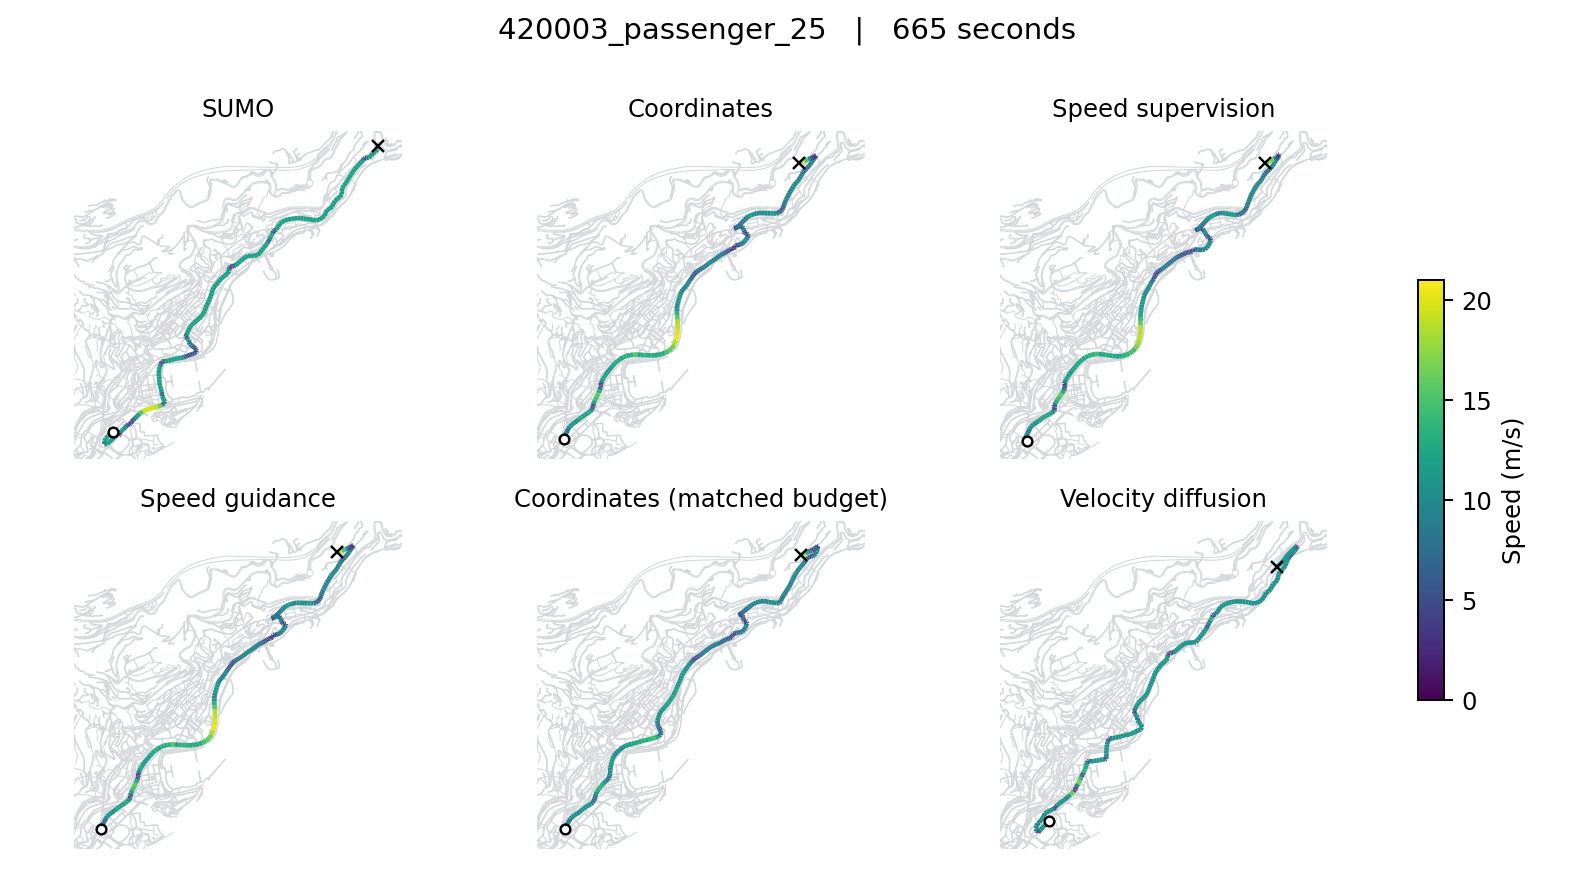
\includegraphics[width=.97\linewidth]{maps/passenger-1.png}\end{center}
\begin{center}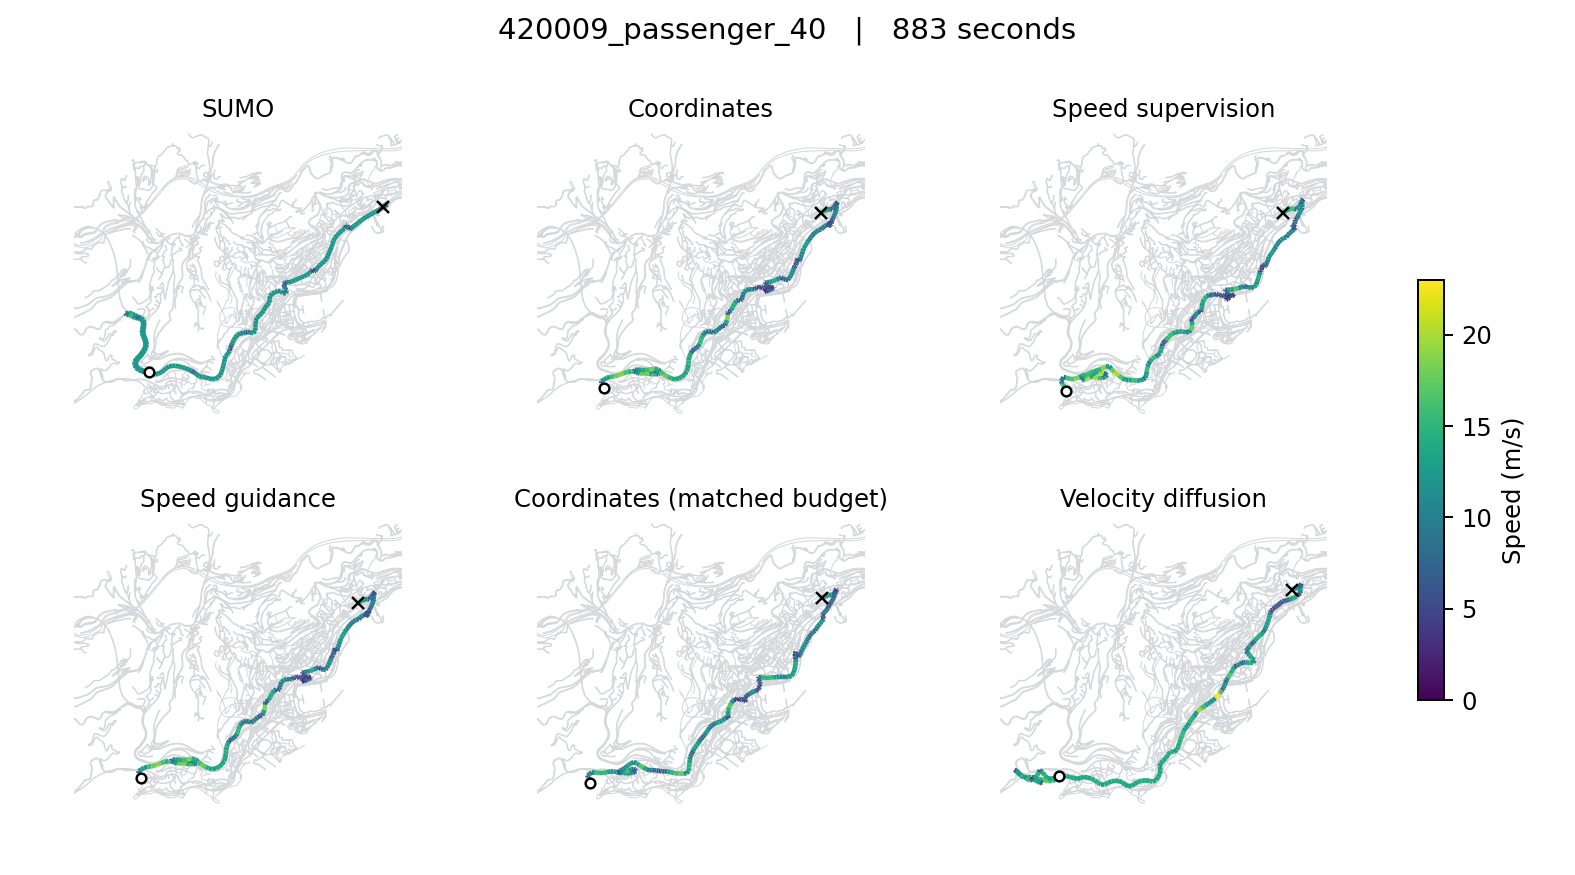
\includegraphics[width=.97\linewidth]{maps/passenger-2.png}\end{center}
{\small Top row: SUMO, coordinate baseline, speed supervision. Bottom row: speed guidance applied to the top-row baseline, the separately trained coordinate control for velocity diffusion, and velocity diffusion. The first two requests per class in the fixed validation order were selected before viewing the maps.}

\newpage\section*{Road maps by vehicle: Taxi}
Each block shows one validation request under the supplied vehicle label (seed 42). Within a block, the six maps share the same road extent and speed scale. A circle marks the start and a cross the end of each plotted path.
\begin{center}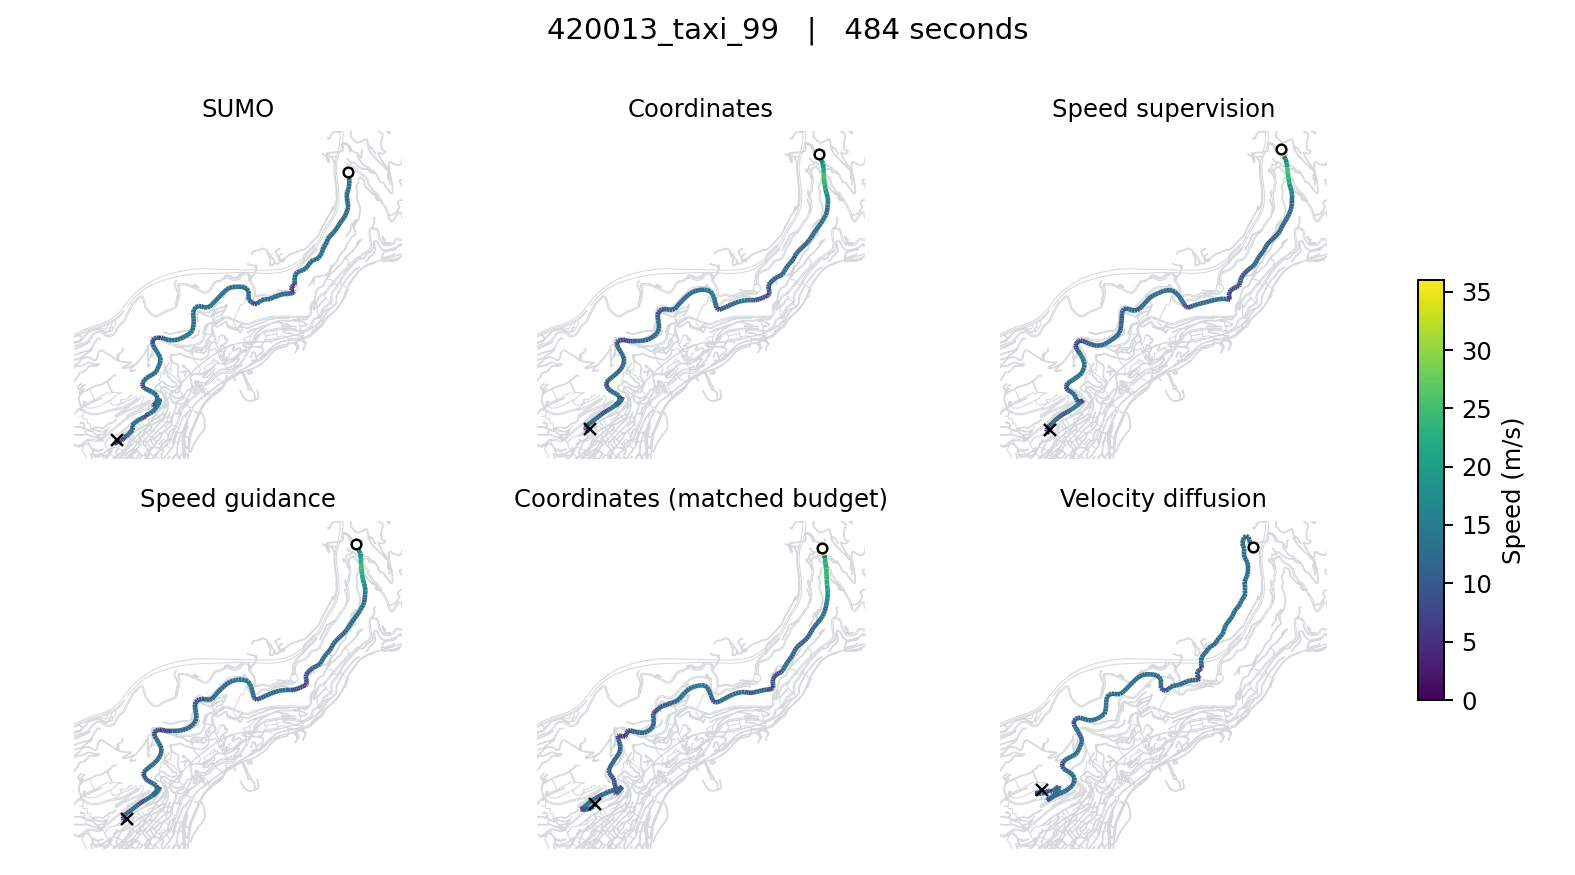
\includegraphics[width=.97\linewidth]{maps/taxi-1.png}\end{center}
\begin{center}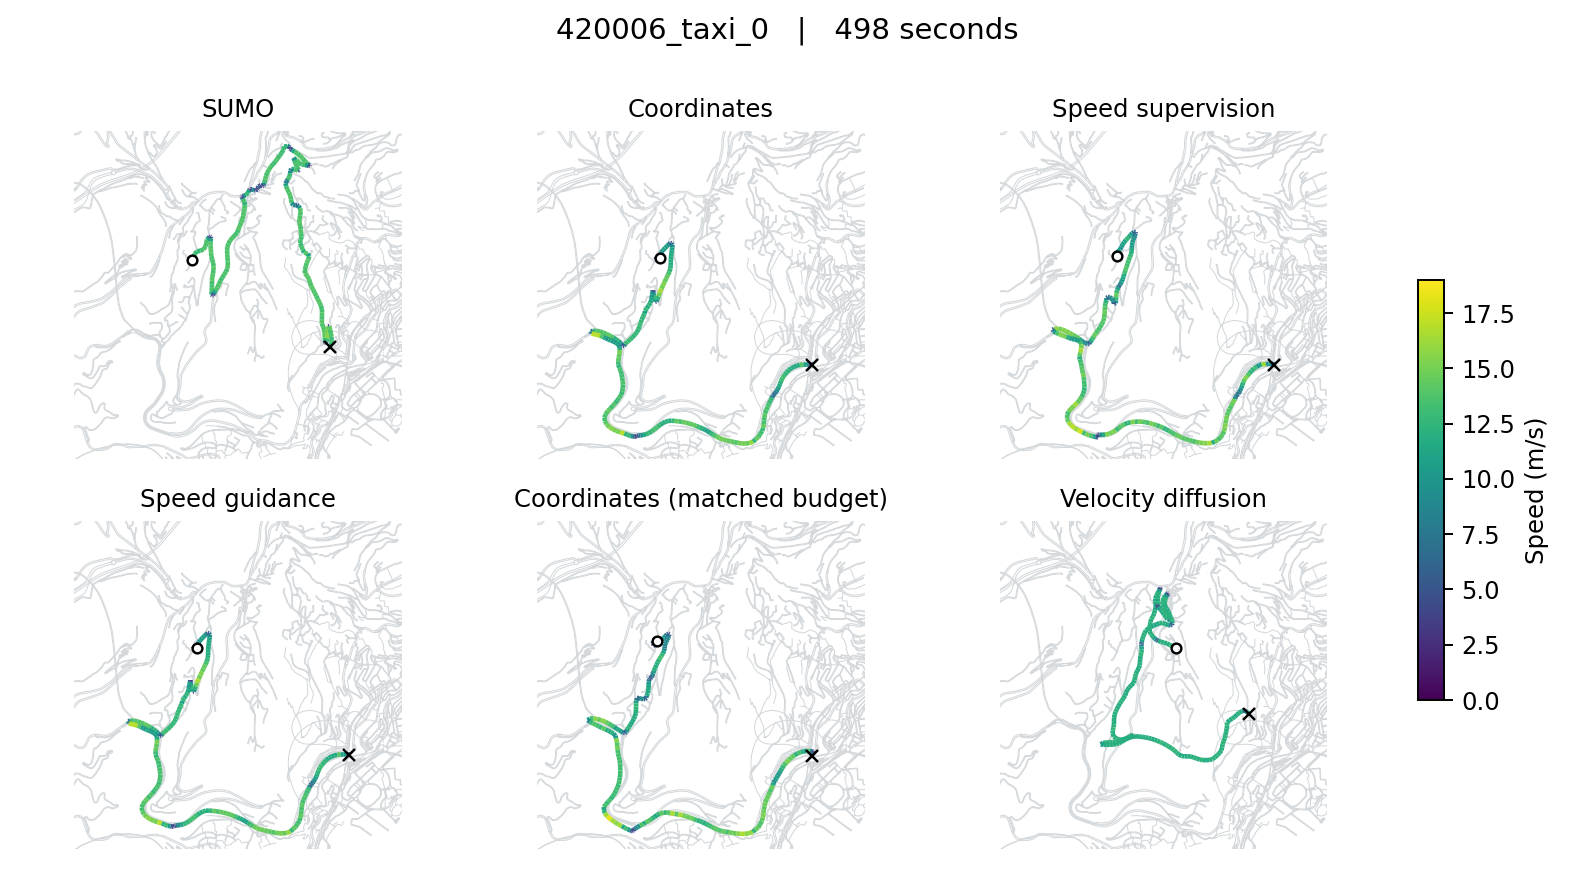
\includegraphics[width=.97\linewidth]{maps/taxi-2.png}\end{center}
{\small Top row: SUMO, coordinate baseline, speed supervision. Bottom row: speed guidance applied to the top-row baseline, the separately trained coordinate control for velocity diffusion, and velocity diffusion. The first two requests per class in the fixed validation order were selected before viewing the maps.}

\end{document}
